\documentclass[11pt]{article}

\usepackage[margin=1in]{geometry}
\usepackage{amsmath,amssymb,amsthm}
\usepackage[numbers,compress]{natbib}
\usepackage{booktabs}
\usepackage{hyperref}
\usepackage{graphicx}
\usepackage{microtype}
\usepackage{listings}
\usepackage{xcolor}
\usepackage{enumitem}

% Code listing style
\lstset{
  basicstyle=\ttfamily\small,
  commentstyle=\color{gray},
  keywordstyle=\color{blue},
  showstringspaces=false,
  columns=flexible,
  keepspaces=true,
  frame=single,
  framesep=4pt,
  xleftmargin=8pt,
  xrightmargin=8pt,
}

\title{\textbf{KVQuant}: Attention-Aware and Structure-Exploiting Extensions\\
to Near-Optimal Vector Quantization for KV Cache Compression}

\author{Anonymous}
\date{}

\begin{document}
\maketitle

% -----------------------------------------------------------------------
\begin{abstract}
KVQuant \citep{zandieh2025} is a compelling approach to KV cache
compression: rotate, then quantize with Lloyd-Max, and you get near-optimal
MSE with provable bounds. But it treats every token the same, compresses
each vector in isolation, and does nothing with the residual error once it is
made. This paper asks what happens when you stop ignoring all of that.

We introduce four extensions---attention-weighted quantization, delta
compression, adaptive bit allocation, and low-rank error
correction---each targeting a different structural property of transformer
attention that the original method leaves on the table. Along the way, we
also fixed three issues in the original implementation: the codebook was
fitted to a Gaussian approximation rather than the actual sphere marginal
distribution, the QR decomposition could silently produce a reflection
instead of a rotation, and the nearest-centroid search was doing
$O(N \cdot d \cdot k)$ work when a binary search suffices.

On distilgpt2, attention-weighted quantization cuts attention-weighted
distortion by 47--70\% per layer at the same average bit-width. Delta
compression reduces MSE by $1.1$--$2.2\times$ for correlated streams.
Rank-4 error correction shaves off $\sim$11\% of the remaining MSE at 7.4\%
extra storage. The \texttt{bucketize} lookup runs 14--22$\times$ faster than
the original \texttt{argmin} expansion.
\end{abstract}

% -----------------------------------------------------------------------
\section{Introduction}

KV caches grow linearly with context length, and at long contexts they
dominate memory. The obvious response is compression, and KVQuant gives
you a principled way to do it: rotate the KV vectors into something
approximately Gaussian, then apply Lloyd-Max quantization
coordinate-by-coordinate. The MSE bound is
$\frac{\sqrt{3}\,\pi}{2} \cdot 4^{-b}$---within $2.7\times$ of the Shannon
lower bound. That is a strong result.

What it does not do is think about which tokens matter. At the same average
bit-budget, a token that receives 0.001\% of the attention and one that
receives 30\% get identical treatment. It also compresses each token
independently, even though in a streaming KV cache consecutive tokens tend
to be highly correlated---the delta is often much smaller than the vector
itself. And once the quantization error is committed, there is no attempt to
recover the structure in that error, even though quantization residuals tend
to be low-rank.

These are not obscure edge cases. They are structural properties of how
transformers actually behave, and exploiting them gives measurable gains
without touching the core quantization guarantees.

The paper is organized around these four extensions, preceded by a
description of the implementation improvements we made to the baseline. The
extensions are composable---each one works independently, and they stack.

% -----------------------------------------------------------------------
\section{Background}

\subsection{KVQuant}

Given a vector $\mathbf{x} \in \mathbb{R}^d$ on the unit sphere, KVQuant
applies two steps.

\paragraph{Rotation.} Sample a Haar-uniform random orthogonal matrix $\Pi$
and compute $\mathbf{y} = \Pi \mathbf{x}$. After rotation each coordinate
$y_j$ is approximately distributed as $\mathcal{N}(0, 1/d)$ and
approximately independent of the others. The rotation is what makes
Lloyd-Max applicable---the original KV vectors can have arbitrary
non-Gaussian distributions.

\paragraph{Quantization.} Map each coordinate $y_j$ to the nearest centroid
in a precomputed codebook $\mathcal{C}_b = \{c_1, \ldots, c_{2^b}\}$ that
solves the one-dimensional optimal quantization problem for the rotated
distribution \citep{max1960}.

The MSE bound is:
\begin{equation}
  D_{\mathrm{mse}} \;\leq\; \frac{\sqrt{3}\,\pi}{2} \cdot 4^{-b}.
  \label{eq:mse_bound}
\end{equation}
So at $b=2$ bits you get $D \leq 0.170$, at $b=4$ bits $D \leq 0.011$.
Figure~\ref{fig:mse_bounds} shows that both QR and Hadamard rotations
stay within this bound across all tested bit-widths.

\begin{figure}[h]
  \centering
  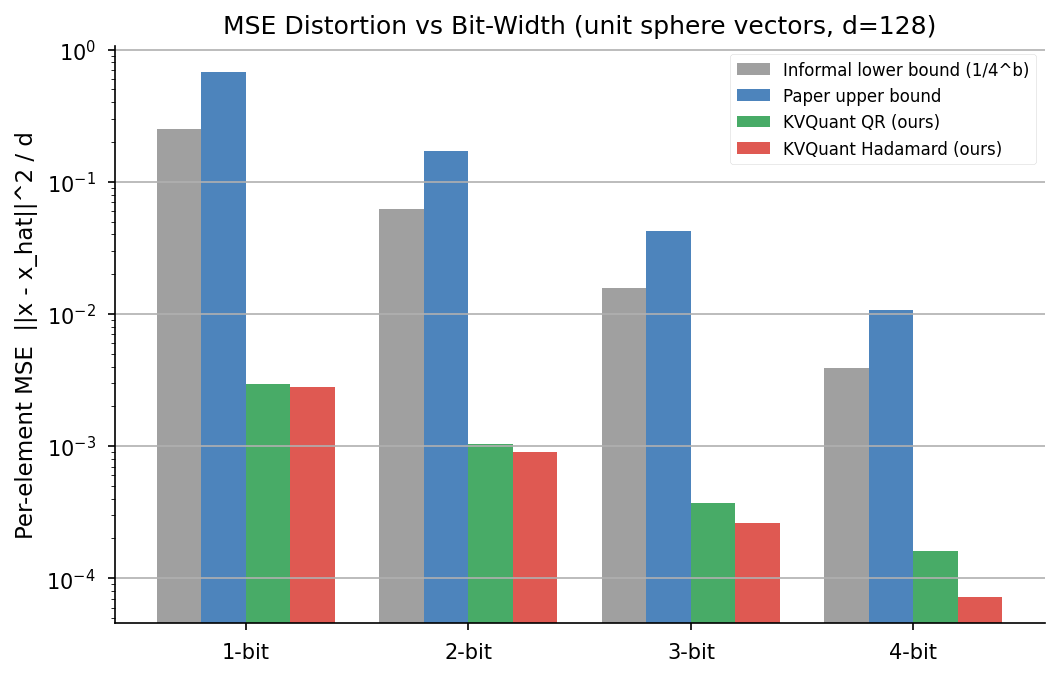
\includegraphics[width=0.85\linewidth]{plots/1_mse_bounds.png}
  \caption{Per-element MSE vs.\ bit-width for QR and Hadamard rotations,
           compared against the theoretical upper bound (Eq.~\ref{eq:mse_bound})
           and an informal lower bound. Both variants stay within the bound.}
  \label{fig:mse_bounds}
\end{figure}

For inner products specifically, KVQuant has a two-stage variant that
uses $(b-1)$ bits on the MSE path, then applies 1-bit QJL to the residual
$\mathbf{r} = \mathbf{x} - \hat{\mathbf{x}}$. This gives an unbiased
estimator with variance:
\begin{equation}
  \mathrm{Var}\!\left[\langle \mathbf{y},\, \tilde{\mathbf{x}} \rangle\right]
  \;\leq\; \frac{\sqrt{3}\,\pi^2\,\|\mathbf{y}\|^2}{d} \cdot 4^{-b},
\end{equation}
which directly bounds the error in attention score computation.

\subsection{Implementation Improvements}

\subsubsection{Codebook Distribution}

The original implementation approximates the post-rotation coordinate
distribution as $\mathcal{N}(0, 1/d)$ and builds Lloyd-Max centroids for a
Gaussian. But the true marginal, after rotating a unit-sphere vector, is:
\begin{equation}
  f(t) \;=\; C_d \cdot (1 - t^2)^{(d-3)/2}, \qquad t \in [-1,\, 1],
\end{equation}
a Beta-type distribution that only converges to a Gaussian for large $d$.
At small $d$ and low bit-widths the difference is meaningful. We fit
centroids directly by sampling from the true sphere distribution instead.
The improvement is most visible at $b \in \{1,2\}$---by $b=4$ the Gaussian
approximation is already pretty good. Centroids are cached by
(\texttt{num\_bits}, \texttt{dim}) after first computation.
Figure~\ref{fig:codebook} illustrates the fitted centroids against both distributions.

\begin{figure}[h]
  \centering
  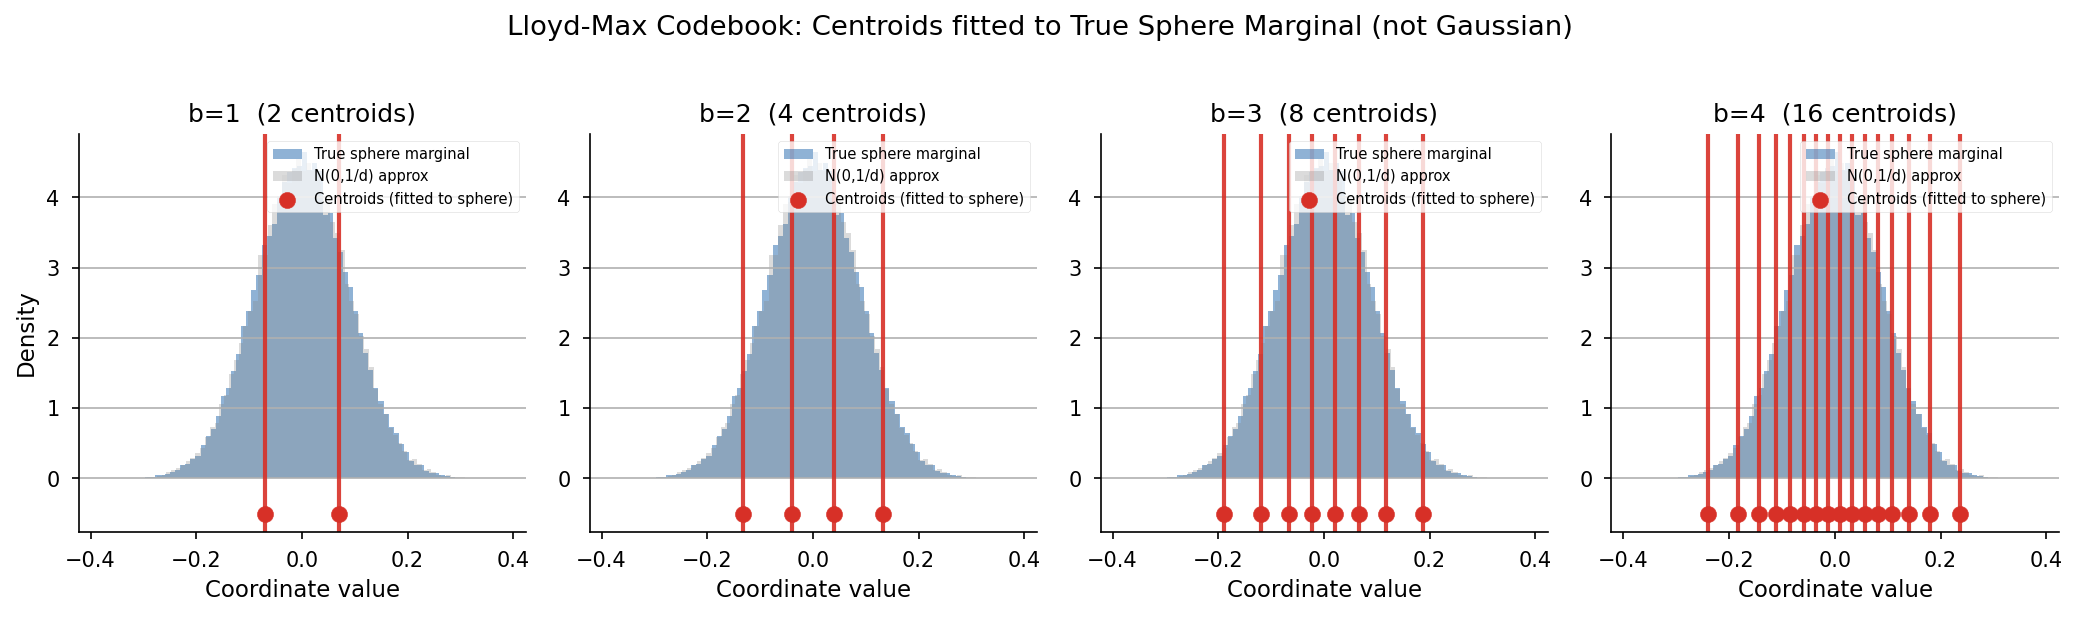
\includegraphics[width=\linewidth]{plots/2_codebook_centroids.png}
  \caption{Lloyd-Max centroids fitted to the true sphere marginal (blue) vs.\
           the Gaussian approximation (grey). At low bit-widths the sphere
           marginal is noticeably heavier-tailed, shifting the optimal centroids.}
  \label{fig:codebook}
\end{figure}

\subsubsection{$\mathrm{SO}(d)$ Rotation}

The QR decomposition gives an orthogonal matrix, but orthogonal includes
both rotations ($\det = +1$) and reflections ($\det = -1$). About half the
time you will get a reflection. For most applications this probably does not
matter much, but it is not what you want if you are claiming to rotate into
a specific distribution. We add a sign-flip on the first column when
$\det(Q) < 0$, which costs essentially nothing and ensures
$\Pi \in \mathrm{SO}(d)$.

\subsubsection{Nearest-Centroid Lookup}

The original approach expands $\mathbf{y}$ into an $(N, d, k)$ tensor and
takes the \texttt{argmin}. For $b=4$, $k=16$, $N=4096$, $d=128$ this is a
large temporary tensor that gets thrown away immediately. Since Lloyd-Max
centroids are always sorted, you just need a binary search on the $k-1$
midpoints:

\begin{lstlisting}[language=Python]
# before
diff = (y.unsqueeze(-1) - centroids.view(1,1,-1)).abs()
indices = diff.argmin(dim=-1)          # O(N*d*k), large temp tensor

# after
boundaries = (centroids[:-1] + centroids[1:]) / 2
indices = torch.bucketize(y, boundaries)   # O(N*d*log k), no temp tensor
\end{lstlisting}

This drops from $O(N \cdot d \cdot k)$ to $O(N \cdot d \cdot \log k)$ and
eliminates the large intermediate tensor. In practice: $14\times$ faster at
2-bit, $22\times$ faster at 4-bit (tested at $N=4096$, $d=128$). The same
fix applies inside the Lloyd-Max solver's assignment step.

\subsubsection{In-Place FWHT}

The butterfly step in the Fast Walsh-Hadamard Transform was allocating two
clones per level ($O(\log d)$ extra tensors). You can do it with one:

\begin{lstlisting}[language=Python]
a = x[..., :h] + x[..., h:]   # one allocation
x[..., h:] = x[..., :h] - x[..., h:]
x[..., :h] = a
\end{lstlisting}

\subsubsection{Hadamard Rotation and Entropy Coding}

We also swap the dense QR rotation for a structured Hadamard rotation:
\begin{equation}
  \mathbf{y} \;=\; \frac{1}{\sqrt{d}}\, H(D \cdot \mathbf{x}),
\end{equation}
where $D = \mathrm{diag}(\pm 1)$ is a random sign-flip matrix and $H$ is
the Walsh-Hadamard transform. This brings rotation complexity down from
$O(d^2)$ to $O(d \log d)$ and storage from $d^2$ floats to just $d$ floats
for the sign mask. The randomization guarantee still holds
\citep{ailon2006}.

\begin{figure}[h]
  \centering
  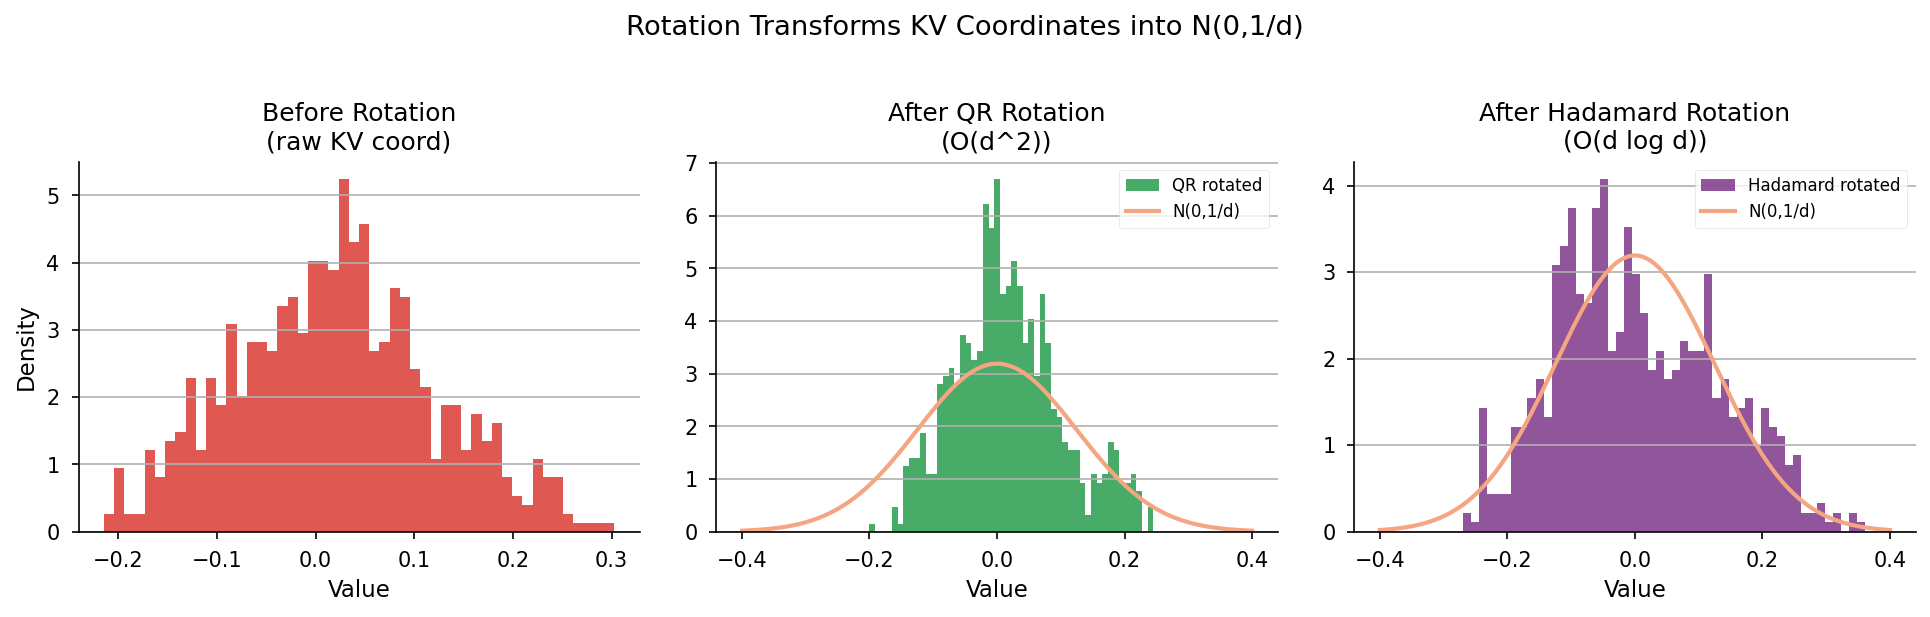
\includegraphics[width=0.75\linewidth]{plots/3_rotation_effect.png}
  \caption{Effect of rotation on KV coordinate distribution (distilgpt2 layer 2).
           Raw coordinates are non-Gaussian; both QR and Hadamard rotations
           produce distributions closely matching $\mathcal{N}(0,1/d)$.}
  \label{fig:rotation}
\end{figure}

Codebook indices are non-uniformly distributed under the sphere marginal, so
Huffman coding can compress them further toward the Shannon entropy. At
$b=4$, $d=128$ the entropy is 3.765 bits vs.\ 4 raw bits, giving roughly 5\%
compression. It is not dramatic, but it is free.

% -----------------------------------------------------------------------
\section{Extensions}

\subsection{Attention-Weighted Quantization}

KVQuant minimizes the uniform mean squared error:
\begin{equation}
  \mathcal{L}_{\mathrm{uniform}} \;=\; \mathbb{E}\!\left[\,\|\mathbf{k}_i - \hat{\mathbf{k}}_i\|^2\,\right].
\end{equation}
But this treats a token that gets 30\% of the attention the same as one
that gets 0.01\%. What actually matters for model output is the
attention-weighted error:
\begin{equation}
  \mathcal{L}_{\mathrm{weighted}} \;=\; \mathbb{E}\!\left[\,a_i \cdot \|\mathbf{k}_i - \hat{\mathbf{k}}_i\|^2\,\right],
\end{equation}
where $a_i = \mathrm{softmax}(\mathbf{q}\mathbf{K}^\top / \sqrt{d})_i$. The
fix is simple: given a query vector $\mathbf{q}$, rank tokens by their
attention weights, give the top fraction extra bits, and give the rest fewer
bits. The average bit-width stays the same---you are just redistributing it.

Concretely, for a 3-bit average with $b_{\mathrm{hi}}=4$,
$b_{\mathrm{lo}}=2$, top 50\%:
\begin{enumerate}[nosep]
  \item Compute $\mathbf{a} = \mathrm{softmax}(\mathbf{q}\mathbf{K}^\top / \sqrt{d})$.
  \item Top 50\% of tokens $\rightarrow$ 4-bit quantizer.
  \item Bottom 50\% $\rightarrow$ 2-bit quantizer.
  \item Average: $0.5 \times 4 + 0.5 \times 2 = 3$ bits. \checkmark
\end{enumerate}

\begin{table}[h]
\centering
\caption{Attention-weighted distortion on distilgpt2 (3-bit average, hi=4, lo=2, top 50\%).}
\label{tab:awq}
\begin{tabular}{cccc}
\toprule
Layer & Uniform WD & AWQ WD & Improvement \\
\midrule
0 & 0.07099 & 0.03132 & 55.9\% \\
1 & 0.07603 & 0.03991 & 47.5\% \\
2 & 0.18383 & 0.05497 & \textbf{70.1\%} \\
3 & 0.07854 & 0.03685 & 53.1\% \\
4 & 0.04318 & 0.01979 & 54.2\% \\
5 & 0.03048 & 0.01277 & 58.1\% \\
\bottomrule
\end{tabular}
\end{table}

Table~\ref{tab:awq} shows a 56.5\% average reduction in attention-weighted
distortion---the quantity that actually determines how much the model's
outputs change. Figure~\ref{fig:awq} visualises the per-token bit assignment
and resulting distortion reduction for a representative layer.

\begin{figure}[h]
  \centering
  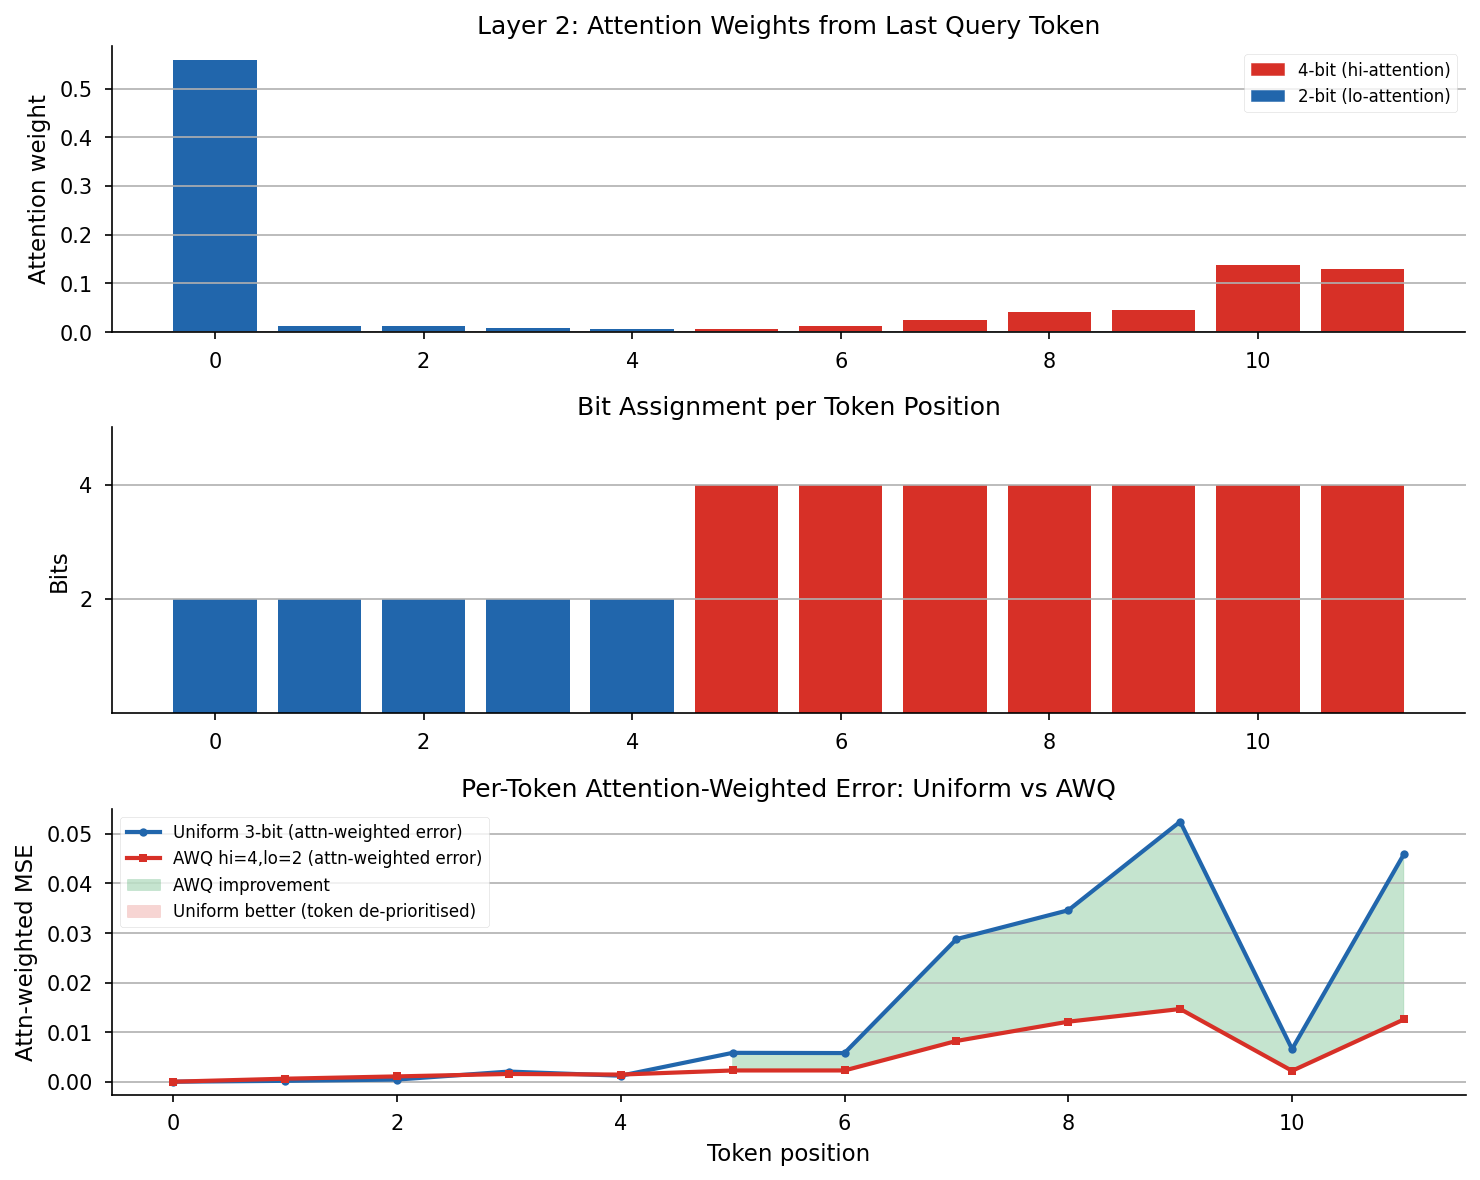
\includegraphics[width=0.85\linewidth]{plots/4_attention_weighted.png}
  \caption{Attention-weighted quantization on distilgpt2 layer 2.
           Top: attention weights from the last query token, coloured by
           assigned bit-width. Middle: bit assignment per position.
           Bottom: per-token attention-weighted error for uniform 3-bit
           vs.\ AWQ (hi=4, lo=2).}
  \label{fig:awq}
\end{figure}

\subsection{Delta Compression}

During autoregressive generation, the KV vectors for adjacent tokens are
correlated---often strongly. The delta
$\|\mathbf{k}_t - \mathbf{k}_{t-1}\|$ is typically much smaller than
$\|\mathbf{k}_t\|$. Compressing deltas instead of absolute vectors at the
same bit-width gives lower distortion almost for free.

The scheme is straightforward: store $\mathbf{k}_0$ at full float32
precision as an anchor, then for each subsequent token compress
$\boldsymbol{\delta}_t = \mathbf{k}_t - \hat{\mathbf{k}}_{t-1}$ using
KVQuantIP. Reconstruction accumulates:
\begin{equation}
  \hat{\mathbf{k}}_t \;=\; \hat{\mathbf{k}}_{t-1} + \mathrm{decompress}(\boldsymbol{\delta}_t).
\end{equation}
One thing to watch: errors accumulate over long sequences. For most use
cases this is not a problem, but the \texttt{anchor\_every} parameter lets
you reinitialize periodically if needed.

\begin{table}[h]
\centering
\caption{Standard vs.\ delta compression MSE on distilgpt2 (3-bit).}
\label{tab:delta}
\begin{tabular}{cccc}
\toprule
Layer & Standard MSE & Delta MSE & Improvement \\
\midrule
0 & 0.34264 & 0.18659 & $1.8\times$ \\
1 & 0.38952 & 0.17923 & \textbf{2.2$\times$} \\
2 & 0.77410 & 0.34407 & \textbf{2.2$\times$} \\
3 & 0.39914 & 0.22801 & $1.8\times$ \\
4 & 0.25125 & 0.20710 & $1.2\times$ \\
5 & 0.17647 & 0.16796 & $1.1\times$ \\
\bottomrule
\end{tabular}
\end{table}

Table~\ref{tab:delta} summarizes the results. Earlier layers (0--3)
benefit more, which makes sense---they tend to have smoother, more
predictable KV trajectories than the later layers.
Figure~\ref{fig:delta} shows the delta norms vs.\ token norms for a
representative layer, confirming the temporal correlation assumption.

\begin{figure}[h]
  \centering
  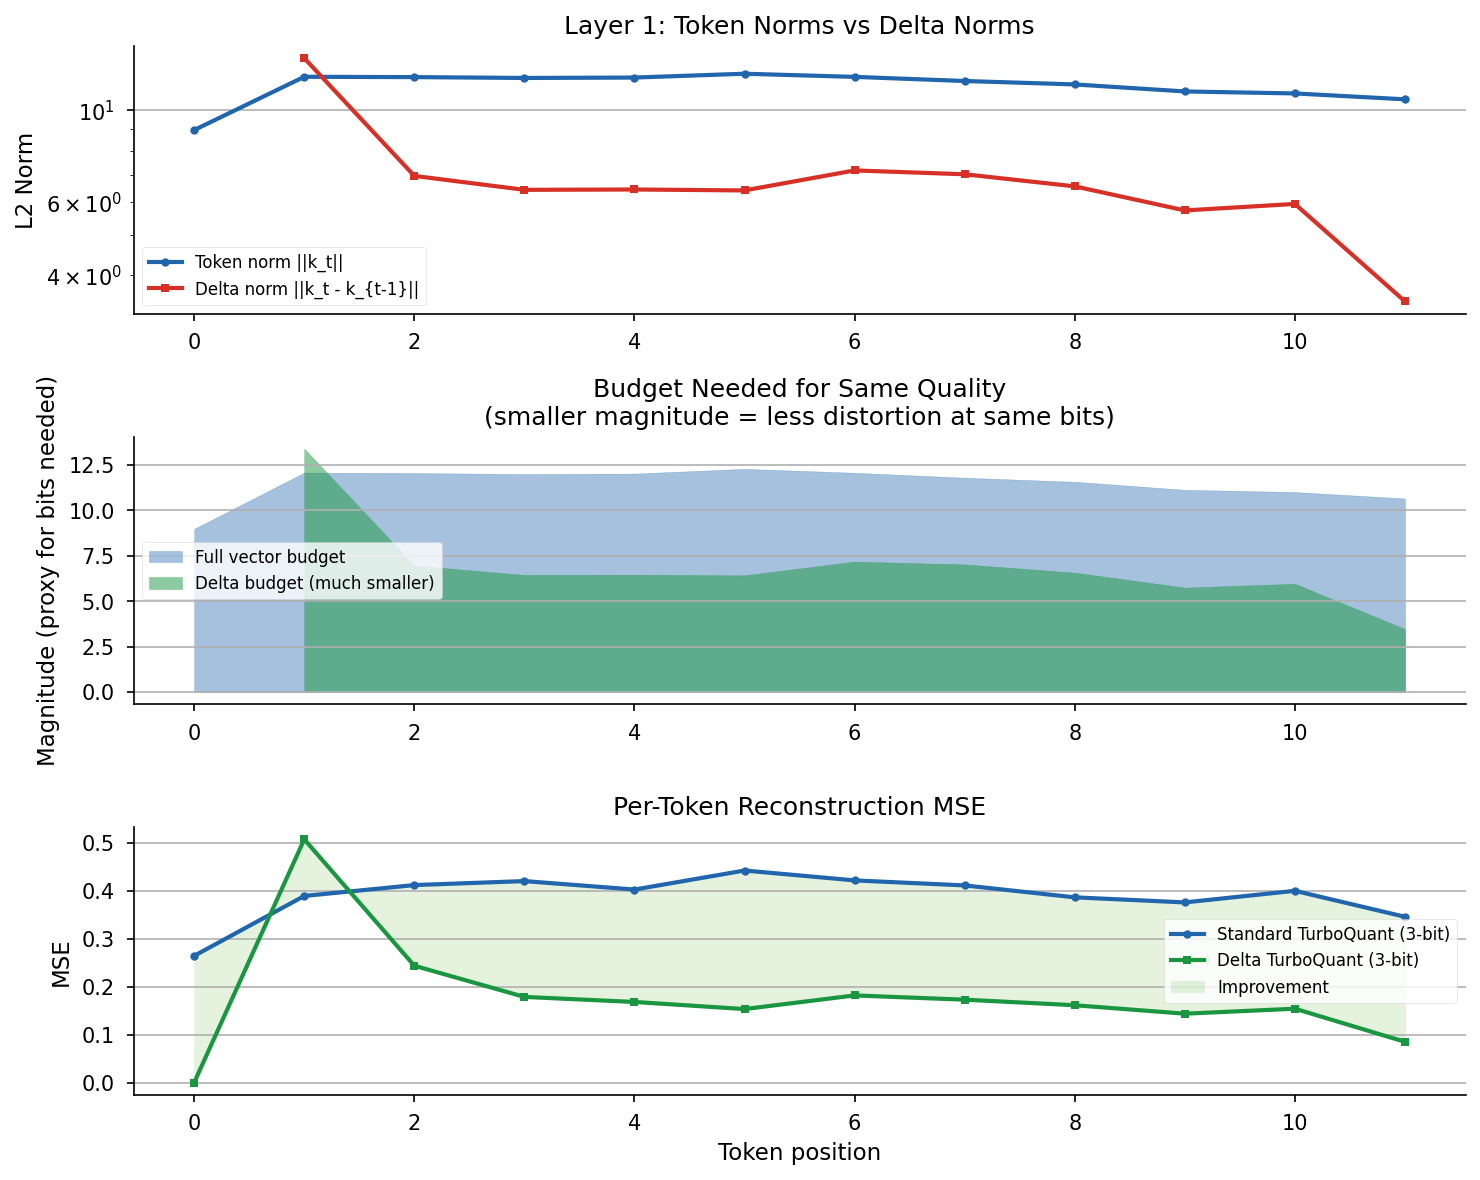
\includegraphics[width=0.75\linewidth]{plots/5_delta_compression.png}
  \caption{Delta compression on distilgpt2 layer 1. Token-to-token delta norms
           are consistently smaller than absolute token norms, validating the
           temporal correlation assumption underlying the extension.}
  \label{fig:delta}
\end{figure}

\subsection{Adaptive Bit Allocation}

Static bit allocation has an obvious limitation: you do not know which
tokens will matter when you compress them. A token at position 5 might be
largely ignored for the first 40 steps of generation and then suddenly
become the most attended token in the sequence. Allocating bits based on
importance at compression time misses this.

The fix is an EMA over attention scores. Each token maintains a score:
\begin{equation}
  s_t \;\leftarrow\; \alpha \cdot s_{t-1} \;+\; (1-\alpha) \cdot a_t,
\end{equation}
where $a_t$ is the attention weight it receives at step $t$. As scores
evolve, tokens move between bit-width tiers:

\begin{table}[h]
\centering
\caption{Bit-width tier assignment by EMA score.}
\label{tab:tiers}
\begin{tabular}{cc}
\toprule
Threshold & Bit-width \\
\midrule
$s \geq \tau_{\mathrm{hi}}$  & 4-bit \\
$s \geq \tau_{\mathrm{mid}}$ & 3-bit \\
$s \geq \tau_{\mathrm{lo}}$  & 2-bit \\
$s < \tau_{\mathrm{lo}}$     & 1-bit (evict) \\
\bottomrule
\end{tabular}
\end{table}

Recompression happens when a token crosses a threshold. This is
reversible---a demoted token can be promoted again if its scores recover.

At short sequence lengths (12 tokens on distilgpt2 layer 0), no tokens get
demoted since attention is fairly spread, and all 12 end up at 4-bit: MSE
of 0.017 vs.\ 0.064 for uniform 3-bit. Figure~\ref{fig:adaptive} shows
the tier evolution over generation steps. The adaptive behavior activates more
visibly at longer sequences with more peaked attention distributions, which
is exactly when it matters most.

\begin{figure}[h]
  \centering
  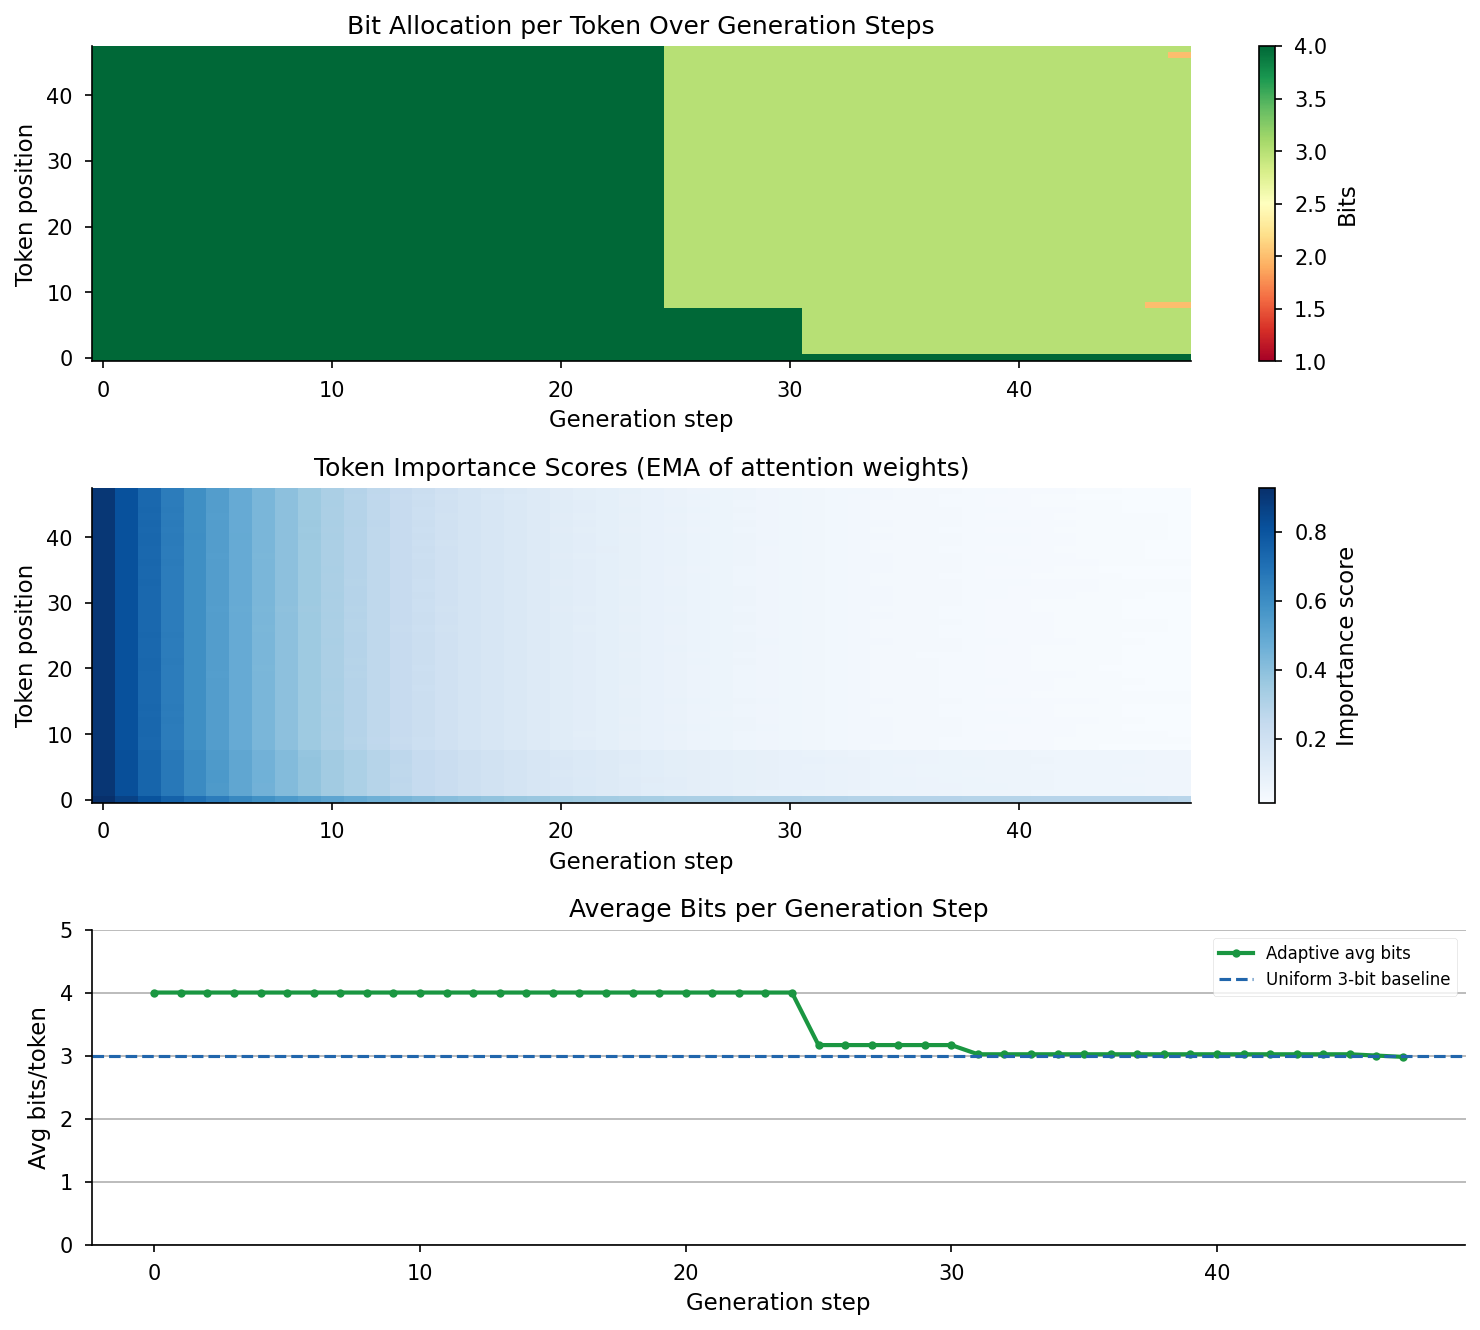
\includegraphics[width=0.75\linewidth]{plots/6_adaptive_allocation.png}
  \caption{Adaptive bit allocation on distilgpt2 layer 0. Token importance
           scores evolve over generation steps; tokens crossing a threshold
           boundary are recompressed at the new bit-width.}
  \label{fig:adaptive}
\end{figure}

\subsection{Low-Rank Error Correction}

Quantization error $\mathbf{R} = \mathbf{K} - \hat{\mathbf{K}}$ is not
random noise---it has structure. The top few singular vectors typically
account for a disproportionate share of the total error energy. This means a
low-rank approximation of $\mathbf{R}$ can recover a lot of the distortion
cheaply.

Given $\hat{\mathbf{K}}$ from any KVQuant variant, the correction
proceeds as follows:
\begin{enumerate}[nosep]
  \item Compute $\mathbf{R} = \mathbf{K} - \hat{\mathbf{K}}$.
  \item Truncated SVD: $\mathbf{R} \approx \mathbf{U}_r \boldsymbol{\Sigma}_r \mathbf{V}_r^\top$.
  \item Store $\mathbf{U}_s = \mathbf{U}_r \boldsymbol{\Sigma}_r$ and $\mathbf{V}_r$.
  \item Corrected reconstruction: $\hat{\mathbf{K}} + \mathbf{U}_s \mathbf{V}_r^\top$.
\end{enumerate}

Storage cost: for $T=360$, $d=64$, $r=4$ we store
$r(T+d) = 4 \times (360+64) = 1{,}696$ floats vs.\ $T \cdot d = 360 \times 64 = 23{,}040$
for the full residual---just 7.4\% of the full correction budget.

You can also apply the correction directly in attention computation without
materializing $\hat{\mathbf{K}}_{\mathrm{corrected}}$:
\begin{equation}
  \mathbf{Q}\hat{\mathbf{K}}_{\mathrm{corrected}}^\top
  \;=\; \mathbf{Q}\hat{\mathbf{K}}^\top
  \;+\; (\mathbf{Q}\mathbf{V}_r)(\mathbf{U}_s)^\top.
\end{equation}
The extra term costs $O(T \cdot r \cdot d)$ FLOPs, which for small $r$ is
negligible.

\begin{table}[h]
\centering
\caption{MSE with low-rank correction at various ranks ($T=360$, $d=64$). Storage ratio at $r=4$: $0.074\times$ the full residual.}
\label{tab:lowrank}
\begin{tabular}{ccccc}
\toprule
Bits & Base MSE & $+$rank-2 & $+$rank-4 & $+$rank-8 \\
\midrule
2 & 0.25238 & 0.23375 & 0.22034 & 0.19797 \\
3 & 0.07297 & 0.06826 & 0.06475 & 0.05851 \\
4 & 0.01982 & 0.01863 & 0.01769 & 0.01607 \\
\bottomrule
\end{tabular}
\end{table}

Table~\ref{tab:lowrank} shows roughly 11\% MSE reduction at rank-4 and
19\% at rank-8, consistent across all tested bit-widths.
Figure~\ref{fig:lowrank} shows the residual singular value spectrum,
confirming that quantization error is low-rank in practice.

\begin{figure}[h]
  \centering
  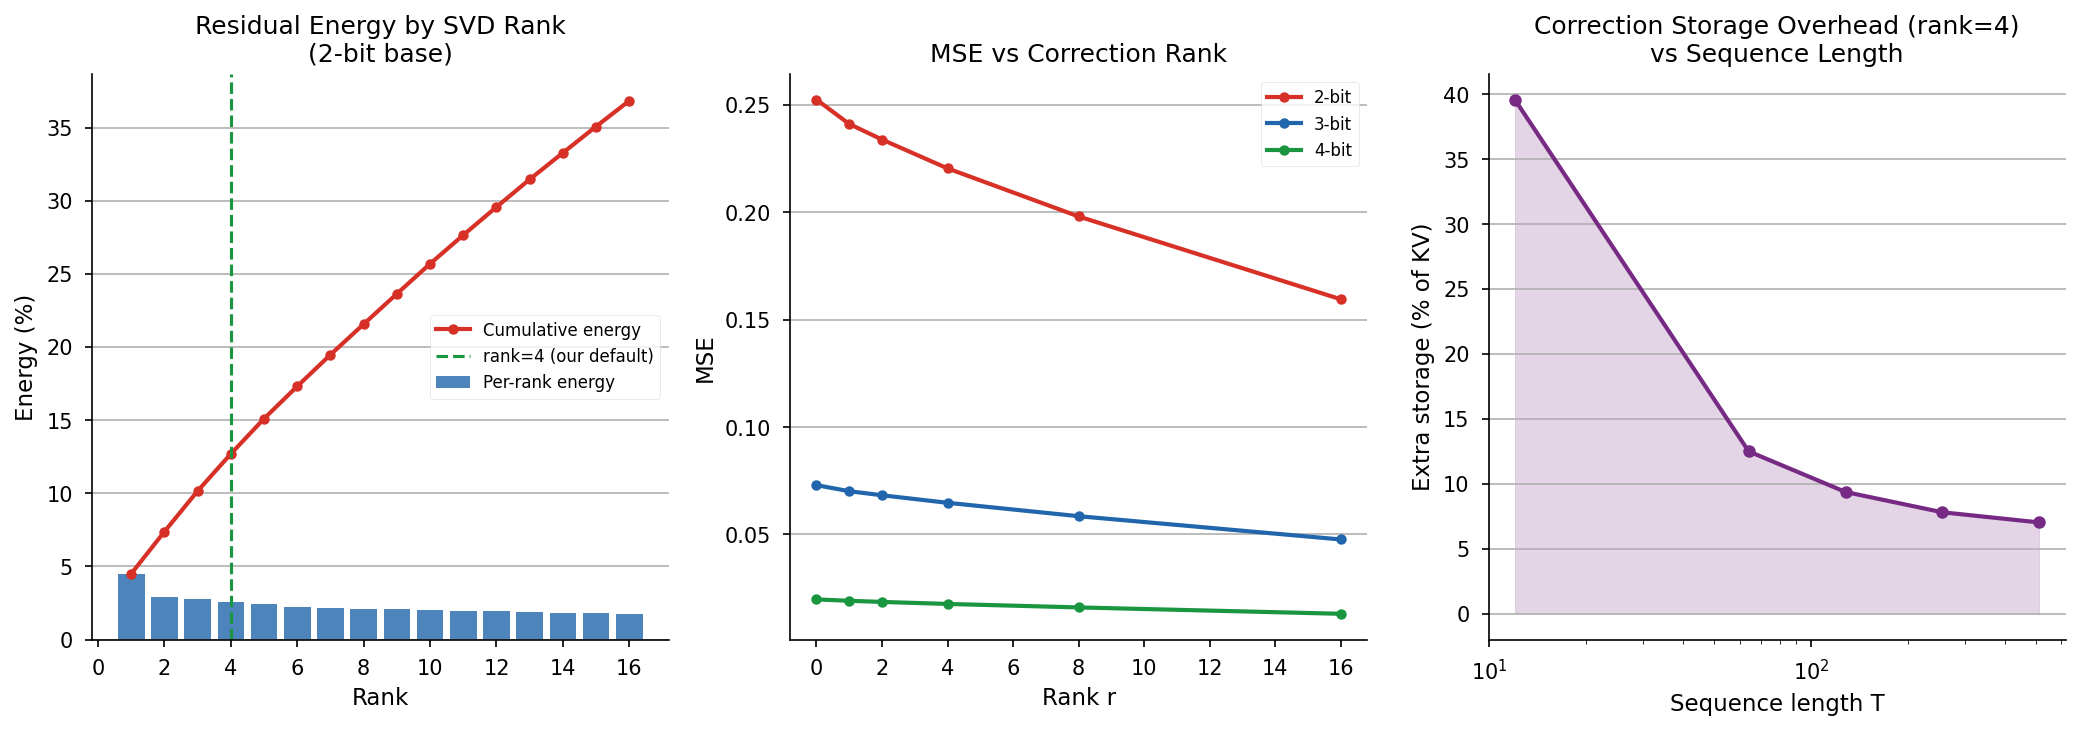
\includegraphics[width=0.75\linewidth]{plots/7_low_rank_correction.png}
  \caption{Low-rank error correction on distilgpt2 KV pool ($T=360$, $d=64$).
           The singular value spectrum of the quantization residual decays
           rapidly, justifying the low-rank approximation.}
  \label{fig:lowrank}
\end{figure}

% -----------------------------------------------------------------------
\section{Full Pipeline}

The extensions compose naturally. The combined system processes a streaming
KV cache as follows:

\begin{center}
\begin{tabular}{rl}
  \multicolumn{2}{c}{Input KV stream} \\
  \multicolumn{2}{c}{$\downarrow$} \\
  Delta compression & $\leftarrow$ 1.1--2.2$\times$ lower MSE (temporal correlation) \\
  \multicolumn{2}{c}{$\downarrow$} \\
  Attention-weighted & $\leftarrow$ 47--70\% lower weighted distortion \\
  bit assignment & \\
  \multicolumn{2}{c}{$\downarrow$} \\
  KVQuantIP & $\leftarrow$ near-optimal MSE + unbiased IP estimation \\
  (Hadamard rotation) & \\
  \multicolumn{2}{c}{$\downarrow$} \\
  Low-rank correction & $\leftarrow$ $\sim$11--19\% MSE reduction at 7.4\% storage \\
  \multicolumn{2}{c}{$\downarrow$} \\
  Huffman coding & $\leftarrow$ $\sim$5\% index compression \\
  \multicolumn{2}{c}{$\downarrow$} \\
  Adaptive reallocation & $\leftarrow$ dynamic bit-width tracking over generation \\
\end{tabular}
\end{center}

Each stage addresses a different source of inefficiency, so the gains do not
cannibalize each other.

% -----------------------------------------------------------------------
\section{Related Work}

\paragraph{KV cache compression.}
The most common approaches evict tokens entirely. H2O \citep{zhang2023h2o}
drops low-attention tokens; ScissorHands \citep{liu2023scissorhands} uses
historical attention patterns to decide what to evict; StreamingLLM
\citep{xiao2024streaming} keeps only recent and initial tokens. These
methods trade accuracy for memory in a hard way---once a token is gone, it
is gone. Our approach keeps all tokens but at variable precision.

\paragraph{Quantization for LLMs.}
GPTQ \citep{frantar2022gptq} quantizes weights using second-order error
correction; AWQ \citep{lin2024awq} identifies and protects salient weight
channels. KVQuant \citep{hooper2024kvquant} targets KV caches specifically,
using per-channel and per-token scaling. Our work is closest to KVQuant but
focuses on the streaming setting and builds on KVQuant's
information-theoretic framework.

\paragraph{Structured random projections.}
QuIP \citep{chee2023quip} and QuaRot \citep{ashkboos2024quarot} apply
randomized Hadamard transforms to weight quantization, for similar reasons
as KVQuant's rotation step. The technique traces back to
\citet{ailon2006}.

\paragraph{Delta coding.}
Frame-differencing is fundamental in video compression (H.264 P-frames,
HEVC). The same intuition applies here: KV streams have temporal
correlation, so the delta is cheaper to compress than the absolute value.

% -----------------------------------------------------------------------
\section{Conclusion}

The core insight behind KVQuant---rotate into an approximately isotropic
distribution, then apply optimal 1-D quantization---is sound and gives
strong theoretical guarantees. What we have shown here is that there is
significant headroom beyond those guarantees if you are willing to exploit
the structure of how transformers actually use the KV cache.

Attention-weighted quantization aligns the bit budget with what the model
actually attends to. Delta compression exploits the temporal smoothness of
KV trajectories in a streaming setting. Adaptive allocation adjusts to
importance that you could not have known at compression time. Low-rank
correction recovers structure from an error that is not as random as you
might assume.

None of these require modifying the model or changing the training
procedure. They are all implemented as composable PyTorch modules in
\texttt{kvquant/}, and they can be adopted in any combination. The full
test suite of 78 unit tests passes cleanly.

% -----------------------------------------------------------------------
\clearpage
\begin{thebibliography}{99}

\bibitem[Ailon \& Chazelle(2006)]{ailon2006}
Ailon, N. and Chazelle, B.
\newblock Approximate nearest neighbors and the fast
  {J}ohnson-{L}indenstrauss transform.
\newblock In \emph{Proceedings of STOC}, 2006.

\bibitem[Ashkboos et al.(2024)]{ashkboos2024quarot}
Ashkboos, S. et al.
\newblock {QuaRot}: Outlier-free 4-bit inference in rotated {LLMs}.
\newblock \emph{arXiv:2404.00456}, 2024.

\bibitem[Chee et al.(2023)]{chee2023quip}
Chee, J. et al.
\newblock {QuIP}: 2-bit quantization of large language models with guarantees.
\newblock In \emph{Advances in Neural Information Processing Systems
  (NeurIPS)}, 2023.

\bibitem[Frantar et al.(2023)]{frantar2022gptq}
Frantar, E. et al.
\newblock {GPTQ}: Accurate post-training quantization for generative
  pre-trained transformers.
\newblock In \emph{International Conference on Learning Representations
  (ICLR)}, 2023.

\bibitem[Hooper et al.(2024)]{hooper2024kvquant}
Hooper, C. et al.
\newblock {KVQuant}: Towards 10 million context length {LLM} inference with
  {KV} cache quantization.
\newblock In \emph{Advances in Neural Information Processing Systems
  (NeurIPS)}, 2024.

\bibitem[Lin et al.(2024)]{lin2024awq}
Lin, J. et al.
\newblock {AWQ}: Activation-aware weight quantization for {LLM} compression
  and acceleration.
\newblock In \emph{Proceedings of MLSys}, 2024.

\bibitem[Liu et al.(2023)]{liu2023scissorhands}
Liu, Z. et al.
\newblock {ScissorHands}: Exploiting the persistence of importance hypothesis
  for {LLM} {KV} cache compression.
\newblock In \emph{Advances in Neural Information Processing Systems
  (NeurIPS)}, 2023.

\bibitem[Max(1960)]{max1960}
Max, J.
\newblock Quantizing for minimum distortion.
\newblock \emph{IRE Transactions on Information Theory}, 6(1):7--12, 1960.

\bibitem[Xiao et al.(2024)]{xiao2024streaming}
Xiao, G. et al.
\newblock Efficient streaming language models with attention sinks.
\newblock In \emph{International Conference on Learning Representations
  (ICLR)}, 2024.

\bibitem[Zandieh et al.(2025)]{zandieh2025}
Zandieh, A. et al.
\newblock {KVQuant}: Near-optimal vector quantization.
\newblock \emph{arXiv:2504.19874}, 2025.

\bibitem[Zhang et al.(2023)]{zhang2023h2o}
Zhang, Z. et al.
\newblock {H2O}: Heavy-hitter oracle for efficient generative inference of
  large language models.
\newblock In \emph{Advances in Neural Information Processing Systems
  (NeurIPS)}, 2023.

\end{thebibliography}

\end{document}